\section{Architectural Design} \label{sec:arch}

This section must give a high-level description of the system in terms of its modules
and their respective purpose and exact interfaces.

\subsection{Architectural Diagram}
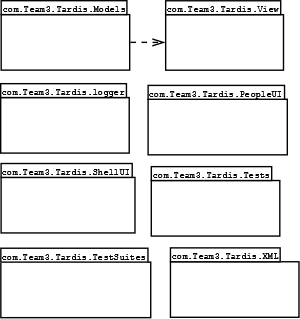
\includegraphics{diagrams/package_diagram}
\\
A UML class diagram or package diagram depicting the high-level structure of the system,
accompanied by a one-paragraph text describing the rationale of this design.
It is mandatory that the system be divided into at least two subsystems,
and that the purpose of each of these subsystems be exposed here.

\subsection{Subsystem Interface Specifications}

Specification of the software interfaces between the subsystems,
i.e. specific messages (or function calls) that are exchanged by the subsystems.
These are also often called ``Module Interface Specifications''.
Description of the parameters to be passed into these function calls in order to have a service fulfilled,
including valid and invalid ranges of values.
Each subsystem interface must be presented in a separate subsection.
